% !TEX encoding = UTF-8 Unicode
% !TEX TS-program = xelatex 
\begin{QUESTIONS}
    \begin{QUESTION}
        \begin{ExamInfo}{100}{學測}{單選}{1}
        \end{ExamInfo}
        \begin{ExamAnsRateInfo}{85}{99}{98}{58}
        \end{ExamAnsRateInfo}
        \begin{QBODY}
			有一箱子,內有 3 黑球與 2 白球。有一遊戲,從箱子中任取出一球。假設每一顆球被取出的機率都相同,若取出黑球可得獎金 50 元,而取出白球可得獎金 100 元,則下 列哪一個選項是此遊戲的獎金期望值?
			\begin{QOPS} 
				\QOP 70 元
				\QOP 75 元 
				\QOP 80 元 
				\QOP 85 元 
				\QOP 90 元
			\end{QOPS}
        \end{QBODY}
        \begin{QFROMS}
        \end{QFROMS}
        \begin{QTAGS}\QTAG{B5C1機率與統計}\end{QTAGS}
        \begin{QANS}
            (1)
        \end{QANS}
        \begin{QSOLLIST}
        \end{QSOLLIST}
        \begin{QEMPTYSPACE}
        \end{QEMPTYSPACE}
    \end{QUESTION}
    \begin{QUESTION}
        \begin{ExamInfo}{100}{學測}{單選}{2}
        \end{ExamInfo}
        \begin{ExamAnsRateInfo}{72}{92}{82}{42}
        \end{ExamAnsRateInfo}
        \begin{QBODY}
			多項式 $4(x^2 +1)+(x+1)^2(x-3)+(x-1)^3$ 等於下列哪一個選項? 
			\begin{QOPS} 
				\QOP $x(x+1)^2$ 
				\QOP $2x(x-1)^2$
				\QOP $x(x-1)(x+1)$    
				\QOP  $2(x-1)^2(x+1)$    
				\QOP $2x(x-1)(x+1)$
			\end{QOPS}
        \end{QBODY}
        \begin{QFROMS}
        \end{QFROMS}
        \begin{QTAGS}\QTAG{B1C2多項式函數}\end{QTAGS}
        \begin{QANS}
            (5)
        \end{QANS}
        \begin{QSOLLIST}
        \end{QSOLLIST}
        \begin{QEMPTYSPACE}
        \end{QEMPTYSPACE}
    \end{QUESTION}
    \begin{QUESTION}
        \begin{ExamInfo}{100}{學測}{單選}{3}
        \end{ExamInfo}
        \begin{ExamAnsRateInfo}{28}{56}{14}{14}
        \end{ExamAnsRateInfo}
        \begin{QBODY}
			設 $(a_{n+1})^2=\frac{1}{\sqrt{10}}(a_n)^2$,$n$ 為正整數,且知 $a_n $ 皆為正。令 $b_n=\log a_n$,則數列 $b_1, b_2,b_3,\cdots,$ 為 
			\begin{QOPS} 
				\QOP 公差為正的等差數列 
				\QOP 公差為負的等差數列 
				\QOP 公比為正的等比數列 
				\QOP 公比為負的等比數列 
				\QOP 既非等差亦非等比數列 。
			\end{QOPS}
        \end{QBODY}
        \begin{QFROMS}
        \end{QFROMS}
        \begin{QTAGS}\QTAG{B1C3指對數函數}\end{QTAGS}
        \begin{QANS}
            (2)
        \end{QANS}
        \begin{QSOLLIST}
        \end{QSOLLIST}
        \begin{QEMPTYSPACE}
        \end{QEMPTYSPACE}
    \end{QUESTION}
    \begin{QUESTION}
        \begin{ExamInfo}{100}{學測}{單選}{4}
        \end{ExamInfo}
        \begin{ExamAnsRateInfo}{30}{51}{20}{19}
        \end{ExamAnsRateInfo}
        \begin{QBODY}
			坐標平面上滿足方程式 $(\frac{x^2}{5^2} + \frac{y^2}{4^2})(\frac{x^2}{3^2} - \frac{y^2}{4^2})=0$ 的點 $(x,y)$ 所構成的圖形為 \quad 
			\begin{QOPS} 
                \QOP 只有原點 
				\QOP 橢圓及原點 
				\QOP 兩條相異直線 
				\QOP 橢圓及雙曲線 
				\QOP 雙曲線及原點
			\end{QOPS}
        \end{QBODY}
        \begin{QFROMS}
        \end{QFROMS}
        \begin{QTAGS}\QTAG{B4C4二次曲線}\end{QTAGS}
        \begin{QANS}
            (3)
        \end{QANS}
        \begin{QSOLLIST}
        \end{QSOLLIST}
        \begin{QEMPTYSPACE}
        \end{QEMPTYSPACE}
    \end{QUESTION}
    \begin{QUESTION}
        \begin{ExamInfo}{100}{學測}{單選}{5}
        \end{ExamInfo}
        \begin{ExamAnsRateInfo}{67}{94}{77}{30}
        \end{ExamAnsRateInfo}
        \begin{QBODY}
		請問下面哪一個選項是正確的? 
		\begin{QOPS} 
			\QOP $3^7 < 7^3$ 
			\QOP $5^{10} < 10^{5}$ 
			\QOP $2^{100} < 10^{30}$ 
			\QOP $\log_2{3} = 1.5$ 
			\QOP $\log_2{11} < 3.5$ 。
		\end{QOPS}
        \end{QBODY}
        \begin{QFROMS}
        \end{QFROMS}
        \begin{QTAGS}\QTAG{B1C3指對數函數}\end{QTAGS}
        \begin{QANS}
            (5)
        \end{QANS}
        \begin{QSOLLIST}
        \end{QSOLLIST}
        \begin{QEMPTYSPACE}
        \end{QEMPTYSPACE}
    \end{QUESTION}
    \begin{QUESTION}
        \begin{ExamInfo}{100}{學測}{單選}{6}
        \end{ExamInfo}
        \begin{ExamAnsRateInfo}{69}{91}{76}{40}
        \end{ExamAnsRateInfo}
        \begin{QBODY}
		根據台灣壽險業的資料,男性從 0 歲、1 歲、...到 60 歲各年齡層的死亡率(單位:$\%$)
		依序為
		1.0250, 0.2350, 0.1520, 0.1010, 0.0720, 0.0590, 0.0550, 0.0540, 0.0540, 0.0520, 0.0490, 0.0470, 0.0490, 0.0560, 0.0759, 0.1029, 0.1394, 0.1890, 0.2034, 0.2123, 0.2164, 0.2166, 0.2137, 0.2085, 0.2019, 0.1948, 0.1882, 0.1830, 0.1799, 0.1793, 0.1813, 0.1862, 0.1941, 0.2051, 0.2190, 0.2354, 0.2539, 0.2742, 0.2961, 0.3202, 0.3472, 0.3779, 0.4129, 0.4527, 0.4962, 0.5420, 0.5886, 0.6346, 0.6791, 0.7239, 0.7711, 0.8229, 0.8817, 0.9493, 1.0268, 1.1148, 1.2139, 1.3250, 1.4485, 1.5851, 1.7353。
		經初步整理後,已知 61 個資料中共有 24 個資料小於 0.2。請問死亡率資料的中位數為下列哪一個選項?
			\begin{QOPS}
				\QOP 0.2034
				\QOP 0.2164
				\QOP 0.2137
				\QOP 0.2085 
				\QOP 0.2019
			\end{QOPS}
        \end{QBODY}
        \begin{QFROMS}
        \end{QFROMS}
        \begin{QTAGS}\QTAG{B2C4數據分析}\end{QTAGS}
        \begin{QANS}
            (2)
        \end{QANS}
        \begin{QSOLLIST}
        \end{QSOLLIST}
        \begin{QEMPTYSPACE}
        \end{QEMPTYSPACE}
    \end{QUESTION}
\end{QUESTIONS}
\begin{QUESTIONS}
    \begin{QUESTION}
        \begin{ExamInfo}{100}{學測}{多選}{7}
        \end{ExamInfo}
        \begin{ExamAnsRateInfo}{40}{73}{32}{15}
        \end{ExamAnsRateInfo}
        \begin{QBODY}
			設 $O$、$A$、$B$ 分別為複數平面上代表 $0$、$1+i$、以及 $1-i$ 的點。請問下列哪些選項所對應的點落在 $\triangle OAB$ 的內部?
			\begin{QOPS} 
				\QOP $\cos 60^\circ$    
				\QOP $\cos 50^\circ +i \sin 50^\circ$    \QOP $\frac{4-3i}{5}$    
				\QOP $\frac{1+\sqrt{3}i}{2}$  
				\QOP $(\cos30^\circ +i\sin 30^\circ) ^{25}$
			\end{QOPS}
        \end{QBODY}
        \begin{QFROMS}
        \end{QFROMS}
        \begin{QTAGS}\QTAG{B5C2三角函數II}\end{QTAGS}
        \begin{QANS}
            (1)(3)(5)
        \end{QANS}
        \begin{QSOLLIST}
        \end{QSOLLIST}
        \begin{QEMPTYSPACE}
        \end{QEMPTYSPACE}
    \end{QUESTION}
    \begin{QUESTION}
        \begin{ExamInfo}{100}{學測}{多選}{8}
        \end{ExamInfo}
        \begin{ExamAnsRateInfo}{54}{82}{55}{25}
        \end{ExamAnsRateInfo}
        \begin{QBODY}
			已知 $\sin \theta = -\frac{2}{3}$ 且 $\cos\theta >0$,請問下列哪些選項是正確的? 
			\begin{QOPS} 
				\QOP $\tan \theta < 0$  
				\QOP $\tan^2\theta > \frac{4}{9}$ 
				\QOP $ \sin^2 \theta > \cos^2 \theta$ 
				\QOP $\sin 2\theta>0$ 
				\QOP 標準位置角 $\theta$ 與 $2\theta$的終邊位在不同的象限
			\end{QOPS}
        \end{QBODY}
        \begin{QFROMS}
        \end{QFROMS}
        \begin{QTAGS}\QTAG{B3C1三角}\end{QTAGS}
        \begin{QANS}
            (1)(2)
        \end{QANS}
        \begin{QSOLLIST}
        \end{QSOLLIST}
        \begin{QEMPTYSPACE}
        \end{QEMPTYSPACE}
    \end{QUESTION}
    \begin{QUESTION}
        \begin{ExamInfo}{100}{學測}{多選}{9}
        \end{ExamInfo}
        \begin{ExamAnsRateInfo}{61}{90}{62}{31}
        \end{ExamAnsRateInfo}
        \begin{QBODY}
			考慮坐標平面上以 $O(0,0)$、$A(3,0)$、$B(0,4)$ 為頂點的三角形,令 $C_1$、$C_2$ 分別為 $\triangle OAB$ 的外接圓、內切圓。請問下列哪些選項是正確的?
			\begin{QOPS}
				\QOP $C_1$ 的半徑為2 
				\QOP $C_1$ 的圓心在直線 $y=x$ 上 
				\QOP $C_1$ 的圓心在直線 $4x+3y=12$ 上    
				\QOP $C_2$ 的圓心在直線 $y=x$ 上 \quad 
				\QOP $C_2$ 的圓心在直線 $4x+3y=6$ 上
			\end{QOPS}
        \end{QBODY}
        \begin{QFROMS}
        \end{QFROMS}
        \begin{QTAGS}\QTAG{B3C2直線與圓}\end{QTAGS}
        \begin{QANS}
            (3)(4)
        \end{QANS}
        \begin{QSOLLIST}
        \end{QSOLLIST}
        \begin{QEMPTYSPACE}
        \end{QEMPTYSPACE}
    \end{QUESTION}
    \begin{QUESTION}
        \begin{ExamInfo}{100}{學測}{多選}{10}
        \end{ExamInfo}
        \begin{ExamAnsRateInfo}{37}{64}{33}{14}
        \end{ExamAnsRateInfo}
        \begin{QBODY}
			坐標平面中,向量 $\lvec{w}$ 與向量 $\lvec{v} = (2,\sqrt{5})$ 互相垂直且等長。請問下列哪些選項是正確的?
			\begin{QOPS} 
				\QOP 向量 $\lvec{w}$ 必為 $(\sqrt{5},-2)$ 或 $(-\sqrt{5},2)$ 
				\QOP 向量$\lvec{v}+\lvec{w}$ 與 $\lvec{v}-\lvec{w}$ 等長 
				\QOP 向量 $\lvec{v}+\lvec{w}$ 與 $\lvec{w}$ 的夾角可能為 $135^\circ$ 
				\QOP 若向量 $\lvec{u}=a \lvec{v}+b \lvec{w}$,其中 $a,b$ 為實數,則向量 $\lvec{u}$ 的長度為 $\sqrt{a^2 +b^2}$ 
				\QOP 若向量 $(1,0)=c\lvec{v}+d \lvec{w}$ , 其中 $c$, $d$ 為實數, 則 $c>0$ 。
			\end{QOPS}
        \end{QBODY}
        \begin{QFROMS}
        \end{QFROMS}
        \begin{QTAGS}\QTAG{B3C3平面向量}\end{QTAGS}
        \begin{QANS}
            (1)(2)(5)
        \end{QANS}
        \begin{QSOLLIST}
        \end{QSOLLIST}
        \begin{QEMPTYSPACE}
        \end{QEMPTYSPACE}
    \end{QUESTION}
    \begin{QUESTION}
        \begin{ExamInfo}{100}{學測}{多選}{11}
        \end{ExamInfo}
        \begin{ExamAnsRateInfo}{47}{76}{46}{19}
        \end{ExamAnsRateInfo}
        \begin{QBODY}
			在坐標平面上,圓 $C$ 的圓心在原點且半徑為 2,已知直線 $L$ 與圓 $C$ 相交,請問 $L$ 與下列哪些圖形一定相交? 
			\begin{QOPS}
				\QOP $x$ 軸 
				\QOP $y = (\frac{1}{2})^x$    
				\QOP  $x^2 +y^2 =3$    \QOP $(x-2)^2 +y^2 =16$ 
				\QOP $\frac{x^2}{9} +\frac{y^2}{4} =1$
			\end{QOPS}
        \end{QBODY}
        \begin{QFROMS}
        \end{QFROMS}
        \begin{QTAGS}\QTAG{B4C4二次曲線}\end{QTAGS}
        \begin{QANS}
            (4)(5)
        \end{QANS}
        \begin{QSOLLIST}
        \end{QSOLLIST}
        \begin{QEMPTYSPACE}
        \end{QEMPTYSPACE}
    \end{QUESTION}
    \begin{QUESTION}
        \begin{ExamInfo}{100}{學測}{多選}{12}
        \end{ExamInfo}
        \begin{ExamAnsRateInfo}{54}{84}{53}{25}
        \end{ExamAnsRateInfo}
        \begin{QBODY}
			坐標空間中,考慮球面 $S:(x-1)^2+(y-2)^2+(z-3)^2 = 14 $ 與 $A(1,0,0)$ 、 $B(-1,0,0)$ 兩點,請問下列哪些選項是正確的? 
			\begin{QOPS} 
				\QOP 原點在球面 $S$ 上 
				\QOP $A$ 點在球面 $S$ 之外部 (3) 線段 $\overline{AB}$ 與球面相交 
				\QOP $A$ 點為直線 $AB$ 上距離球心最近的點  
				\QOP 球面 $S$ 和 $xy$, $yz$, $xz$ 平面分別截出的三個圓中,以與 $xy$ 平面所截的圓面積最大。
			\end{QOPS}
        \end{QBODY}
        \begin{QFROMS}
        \end{QFROMS}
        \begin{QTAGS}\QTAG{B4C1空間向量}\end{QTAGS}
        \begin{QANS}
            (1)(3)(4)
        \end{QANS}
        \begin{QSOLLIST}
        \end{QSOLLIST}
        \begin{QEMPTYSPACE}
        \end{QEMPTYSPACE}
    \end{QUESTION}
    \begin{QUESTION}
        \begin{ExamInfo}{100}{學測}{多選}{13}
        \end{ExamInfo}
        \begin{ExamAnsRateInfo}{39}{64}{32}{21}
        \end{ExamAnsRateInfo}
        \begin{QBODY}
		設 $f(x) = x(x -1)(x +1)$ ,請問下列哪些選項是正確的? 
			\begin{QOPS} 
				\QOP $f(\frac{1}{\sqrt{2}})>0$

				\QOP $f(x)=2$ 有整數解

				\QOP $f(x)=x^2+1$ 有實數解

				\QOP  $f(x) = x$ 有不等於零的有理數解 
				\QOP 若 $f(a)=2$,則 $f(-a)=2$
			\end{QOPS}
        \end{QBODY}
        \begin{QFROMS}
        \end{QFROMS}
        \begin{QTAGS}\QTAG{B1C2多項式函數}\end{QTAGS}
        \begin{QANS}
            (3)
        \end{QANS}
        \begin{QSOLLIST}
        \end{QSOLLIST}
        \begin{QEMPTYSPACE}
        \end{QEMPTYSPACE}
    \end{QUESTION}
\end{QUESTIONS}
\begin{QUESTIONS}
    \begin{QUESTION}
        \begin{ExamInfo}{100}{學測}{填充}{A}
        \end{ExamInfo}
        \begin{ExamAnsRateInfo}{49}{92}{50}{5}
        \end{ExamAnsRateInfo}
        \begin{QBODY}
				已知首項為 $a$、公比為 $r$ 的無窮等比級數和等於5;首項為 $a$、公比為 $3r$ 的無窮等比級數和等於 7 ,則首項為 $a$ 、公比為 $2r$ 的無窮等比級數和等於 $\TCNBOX{\FR{\TCN\TCN}{\TCN}}$ 。 
        \end{QBODY}
        \begin{QFROMS}
        \end{QFROMS}
        \begin{QTAGS}\QTAG{B6C1函數與極限}\end{QTAGS}
        \begin{QANS}
            $\frac{35}{6}$
        \end{QANS}
        \begin{QSOLLIST}
        \end{QSOLLIST}
        \begin{QEMPTYSPACE}
        \end{QEMPTYSPACE}
    \end{QUESTION}
    \begin{QUESTION}
        \begin{ExamInfo}{100}{學測}{填充}{B}
        \end{ExamInfo}
        \begin{ExamAnsRateInfo}{55}{92}{61}{12}
        \end{ExamAnsRateInfo}
        \begin{QBODY}
		空間中一長方體如下圖所示,其中 $ABCD$ 為正方形,$\overline{BE}$ 為長方體的一邊。已知 $\cot \angle AEB = \frac{2\sqrt{6}}{5}$ ,則 $\cot \angle CED = \TCNBOX{\FR{\TCN}{\TCN}}$ 

			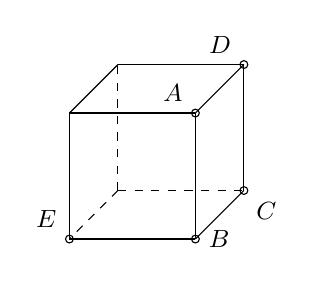
\begin{tikzpicture}
			\begin{scope}[scale=.8] \small
			\draw[dashed] (0,0,0) -- (2,0,0);
			\draw[dashed] (0,0,0) -- (0,2,0);
			\draw[dashed] (0,0,0) -- (0,0,2);
			\draw (2,0,0) -- (2,2,0);
			\draw (2,0,0) -- (2,0,2);
			\draw (0,2,0) -- (0,2,2);
			\draw (0,2,0) -- (2,2,0);
			\draw (0,0,2) -- (0,2,2);
			\draw (0,0,2) -- (2,0,2);
			\draw (2,2,0) -- (2,2,2);
			\draw (2,0,2) -- (2,2,2);
			\draw (0,2,2) -- (2,2,2);
			\tikzstyle{vnode}=[draw, circle, inner sep=1pt];
			\node[vnode] (A) at (2,2,2) [label=150:$A$] {};
			\node[vnode] (B) at (2,0,2) [label=0:$B$] {};
			\node[vnode] (C) at (2,0,0) [label=-40:$C$] {};
			\node[vnode] (D) at (2,2,0) [label=150:$D$] {};
			\node[vnode] (E) at (0,0,2) [label=150:$E$] {};
			\end{scope}
			\end{tikzpicture}

        \end{QBODY}
        \begin{QFROMS}
        \end{QFROMS}
        \begin{QTAGS}\QTAG{B4C1空間向量}\end{QTAGS}
        \begin{QANS}
            $\frac{5}{7}$
        \end{QANS}
        \begin{QSOLLIST}
        \end{QSOLLIST}
        \begin{QEMPTYSPACE}
        \end{QEMPTYSPACE}
    \end{QUESTION}
    \begin{QUESTION}
        \begin{ExamInfo}{100}{學測}{填充}{C}
        \end{ExamInfo}
        \begin{ExamAnsRateInfo}{46}{82}{50}{6}
        \end{ExamAnsRateInfo}
        \begin{QBODY}
			高三甲班共有 20 位男生、15位女生,需推派3位同學參加某項全校性活動。班會中大家決定用抽籤的方式決定參加人選。若每個人中籤的機率相等,則推派的三位同學中有男也有女的機率為 $\TCNBOX{\FR{\TCN\TCN}{\TCN\TCN\TCN}}$ 。
        \end{QBODY}
        \begin{QFROMS}
        \end{QFROMS}
        \begin{QTAGS}\QTAG{B2C3機率}\end{QTAGS}
        \begin{QANS}
            $\frac{90}{119}$
        \end{QANS}
        \begin{QSOLLIST}
        \end{QSOLLIST}
        \begin{QEMPTYSPACE}
        \end{QEMPTYSPACE}
    \end{QUESTION}
    \begin{QUESTION}
        \begin{ExamInfo}{100}{學測}{填充}{D}
        \end{ExamInfo}
        \begin{ExamAnsRateInfo}{32}{73}{21}{2}
        \end{ExamAnsRateInfo}
        \begin{QBODY}
			四邊形 $ABCD$ 中, $AB=1$, $BC=5$, $CD=5$, $DA=7$,且 $\angle DAB= \angle BCD=90^\circ$,則對角線 $\overline{AC}$ 長為 $\TCNBOX{\TCN\TCN}$。
        \end{QBODY}
        \begin{QFROMS}
        \end{QFROMS}
        \begin{QTAGS}\QTAG{B3C1三角}\end{QTAGS}
        \begin{QANS}
            $\sqrt{32}$
        \end{QANS}
        \begin{QSOLLIST}
        \end{QSOLLIST}
        \begin{QEMPTYSPACE}
        \end{QEMPTYSPACE}
    \end{QUESTION}
    \begin{QUESTION}
        \begin{ExamInfo}{100}{學測}{填充}{E}
        \end{ExamInfo}
        \begin{ExamAnsRateInfo}{26}{59}{17}{2}
        \end{ExamAnsRateInfo}
        \begin{QBODY}
			一礦物內含 $A$、$B$、$C$ 三種放射性物質,放射出同一種輻射。已知 $A$、$B$、$C$ 每公克分別會釋放出 1 單位、2 單位、1 單位的輻射強度,又知 $A$ 、 $B$ 、 $C$ 每過半年其質量分別變為原來質量的  $\frac{1}{2}$ 、 $\frac{1}{3}$ 、 $\frac{1}{4}$ 倍。於一年前測得此礦物的輻射強度為 66 單位,而半年前測得此礦物的輻射強度為 22 單位,且目前此礦物的輻射強度為 8 單位,則目前此礦物中 $A$、$B$、$C$ 物質之質量分別為 $\TCNBOX{\TCN}$ 、 $\TCNBOX{\TCN}$ 、 $\TCNBOX{\TCN}$ 公克。
        \end{QBODY}
        \begin{QFROMS}
        \end{QFROMS}
        \begin{QTAGS}\QTAG{B4C3矩陣}\end{QTAGS}
        \begin{QANS}
            $4,1,2$
        \end{QANS}
        \begin{QSOLLIST}
        \end{QSOLLIST}
        \begin{QEMPTYSPACE}
        \end{QEMPTYSPACE}
    \end{QUESTION}
    \begin{QUESTION}
        \begin{ExamInfo}{100}{學測}{填充}{F}
        \end{ExamInfo}
        \begin{ExamAnsRateInfo}{27}{66}{14}{1}
        \end{ExamAnsRateInfo}
        \begin{QBODY}
			設 $E_1:  \frac{x^2}{a^2} +\frac{y^2}{b^2} =1$ (其中 $a>0$ ) 為焦點在 $(3,0)$, $(-3,0)$ 的橢圓;$E_2$ :焦點在 $(3, 0)$ 且準線為 $x = -3$ 的拋物線。 已知 $E_1, E_2$ 的交點在直線 $x=3$ 上,則 $a=\TCNBOX{\TCN+\TCN\sqrt{\TCN}}$。
        \end{QBODY}
        \begin{QFROMS}
        \end{QFROMS}
        \begin{QTAGS}\QTAG{B4C4二次曲線}\end{QTAGS}
        \begin{QANS}
            $3+3\sqrt{2}$
        \end{QANS}
        \begin{QSOLLIST}
        \end{QSOLLIST}
        \begin{QEMPTYSPACE}
        \end{QEMPTYSPACE}
    \end{QUESTION}
    \begin{QUESTION}
        \begin{ExamInfo}{100}{學測}{填充}{G}
        \end{ExamInfo}
        \begin{ExamAnsRateInfo}{31}{74}{17}{2}
        \end{ExamAnsRateInfo}
        \begin{QBODY}
			$H: x-y+z=2$ 為坐標空間中一平面,$L$ 為平面 $H$ 上的一直線。已知點 $P(2,1,1)$ 為 $L$ 上距離原點 $O$ 最近的點,則 $\TCNBOX{(\TCN,\TCN\TCN,\TCN\TCN)}$ 為 $L$ 的方向向量。
        \end{QBODY}
        \begin{QFROMS}
        \end{QFROMS}
        \begin{QTAGS}\QTAG{B4C1空間向量}\end{QTAGS}
        \begin{QANS}
            $(2,-1,-3)$
        \end{QANS}
        \begin{QSOLLIST}
        \end{QSOLLIST}
        \begin{QEMPTYSPACE}
        \end{QEMPTYSPACE}
    \end{QUESTION}
\end{QUESTIONS}
